\documentclass{article}
\usepackage[margin=0.8in]{geometry}
\usepackage{amsmath, amssymb}
\usepackage{hyperref}
\usepackage{graphicx}
\usepackage{bm}

\graphicspath{{figs/}}


\title{Hints, Clues and Excerpts}
\date{November 23, 2022}
\author{Rishav}

\begin{document}
\maketitle
\begin{center}
  Last modified: \today{} 
\end{center}
\tableofcontents
\newpage

\section{Mean of a random variable on a manifold}
\href{https://djalil.chafai.net/blog/2010/05/01/mean-of-random-variable-on-manifold/}{Djalil Chafai (May 1, 2010)} \\

Let $\bm{X}$ be a random variable on a manifold $\bm{M}$. Is there a nice (intrinsic?) definition of a mean of $\bm{X}$ and of its variance? This funny question comes from concrete motivations (imaging). What can be done with a chart? The problem here is that the mean is a global notion.\medskip

If $\bm{M}$ has global coordinates of almost global, like stereographical projections for spheres, one may use them. This is ugly and non canonical. If $\bm{M}$ is a Lie group, one may use the exponential map. When $M$ is equipped with a Riemannian metric $d: \bm{M}\times \bm{M} \rightarrow\mathbb{R}_{+}$ one may think about using a variational approach, and simply define the mean $m$ of $\bm{X}$ as

$$
  m:=\text{arg}\,\min\limits_{x\in\bm{M}}\, \mathbb{E}(d(x, \bm{X})^{2}).
$$

The value of minimum is the variance of $\bm{X}$. This definition does not always provide unique point on $\bm{M}$, as shown by the example of the uniform law on spheres for which every point is a mean! This is not a bug, it is a feature, a geometrical feature due to the invariance of the law by isometries in this example. One can ask about an empirical estimator of mean, and its asymptotic fluctuations. For some answers, see e.g. the work of Pennec and Bhattacharya and Bhattacharya. The variational expression of $d$ in terms of geodesics is valid up to the cut-locus/injectivity-radius of the exponential map.\medskip

Beyond the mean, the law of $\bm{X}$ may be viewed as the linear from
$$
  f \in \mathcal{C}_{b}(\bm{M}, \mathbb{R})\mapsto \mathbb{E}(f(\bm{X})).
$$

This does not rely on the manifold nature of $\bm{M}$ since we only use the fact that $\bm{M}$ is a topological space. Note that if $\bm{M}$ is an open subset of $\mathbb{R}^{d}$ then we recover the usual $\mathbb{E}(\bm{X})$ by the approximation via dominated convergence. The integrability of $\bm{X}$ is the class of functions for which the map above is finite. In some sense $\mathbb{E}(\bm{X})$ is an element of the bidual $\bm{M}''$  of $\bm{M}$, provided that we view  $M':=\mathcal{C}_{b}(\bm{M},\mathbb{R})$ as a sort of dual of $\bm{M}$. Of course, $\bm{M}\subset\bm{M}''$ via the canonical injection but the converse does not hold in general. \medskip

If $(\bm{X}_{n})_{n\ge 0}$ is an irreducible positive recurrent aperiodic Marcov chain with state space $M$ and unique invariance law $\mu$ then the large numbers of states that with probability one, and regardless of the initial law of the chain, we have

$$
  \frac{1}{n}\delta_{\bm{X}_{1}} + ... + \frac{1}{n}\delta_{\bm{X}_{n}}\xrightarrow[n\rightarrow \infty]{\mathcal{C}_{b}(\bm{M},\mathbb{R})}\mu.
$$

The asymptotic fluctuations of this convergence are described by the central limit theorem, which involves the variance of $\mu$ of the solution of the Poisson equation associated to the dynamics.

\section{Sequential Optimal Attitude Recursion Filter}
\href{https://arc.aiaa.org/doi/10.2514/1.49561}{Christian and Lightsey (2010)}\\

Note that all of the SOAR filter update equations make the assumptions that the a priori state error and measurement error have Gaussian distributions. The equations of motion for attitude propagation are nonlinear and it is well-known that Gaussian distribution undergoing a nonlinear transformation do not necessarily remain Gaussian. Therefore, it is unlikely that the a priori state error at any given time is truly Gaussian. Despite the face that the true underlying distribution may not actually be Gaussian, many filters still assume a Gaussian distribution. Empirical evidence has shown that these filters still perform well in many scenarios, even though the simplifying assumption of a Gaussian distribution may not strictly be true.

\section{What is the Covariance Matrix?}
\href{https://fouryears.eu/2016/11/23/what-is-the-covariance-matrix/}{Konstantin (Novemver 23, 2016)}\\

Most textbooks on statistics cover covariance right in their first chapters. It is defined as a useful "measure of dependency" between two random variables:

$$
  \text{cov}(X, Y) = \mathbb{E}[(X - \mathbb{E}[X])(Y-\mathbb{E}[Y])].
$$

The textbook would usually provide some intuition on why it is defined as it is, prove a couple of properties, such as bilinearity, define the \textit{covariance matrix} for multiple variable as $\Sigma_{ij} = \text{cov}(X_{i},Y_{j})$ and stop there. Later on the covariance matrix would pop up here and there in seemingly random ways. In one place you would have to take its inverse, in another compute the eigenvectors or multiply a vector by it, or do something else for no apparent reason apart from "that's the solution we came up with by solving an optimization task".\,medskip

In reality though, there are some very good and quite intuitive reasons for why the covariance matrix appears in various techniques in one or other way. This post aims to show that, illustrating some curious corners of linear algebra in the process.

\paragraph{Meet the Normal Distribution}\mbox{}\\\\
The best way to truly understand the covariance matrix is to forget the textbook definitions completely and depart from a different point instead Namely, from the definition of the multivariate Gaussian distribution.\medskip

We say that the vector $\bm{x}$ has a \textit{normal} (or \textit{Gaussian}) distribution with mean $\mu$ and covariance $\Sigma$ if:

$$
 \text{Pr}(\bm{x}) = \big|2\pi\Sigma\big|^{\frac{1}{2}} \exp\left(-\frac{1}{2}(\bm{x}-\mu)^{\intercal}\Sigma^{-1}(\bm{x}-\mu)\right).
$$

To simplify the math a bit, we will limit ourselves to the centered distribution (i.e. $\mu = \bm{0}$) and refrain from writing the normalizing constant $\big|2\pi\Sigma\big|^{\frac{1}{2}}$. Now, the definition of the (centered) multivariate Gaussian looks as follows:

$$
  \text{Pr}(\bm{x})\propto\exp\left(-0.5\,\bm{x}^{\intercal}\Sigma^{-1}\bm{x}\right)
$$

Much simpler, isn't it? Finally, let us define the covariance matrix as nothing else but \textit{the parameter of the Gaussian distribution}. That's it. You will see where it lead us in a moment.

\paragraph{Transforming the Symmetric Gaussian}\mbox{}\\\\
Consider a symmetric Gaussian distribution, i.e. the one with $\Sigma = \bm{I}$ (the identity matrix). Let us take a sample form it, which will of course be symmetric, round cloud of points:
 
\begin{center}
  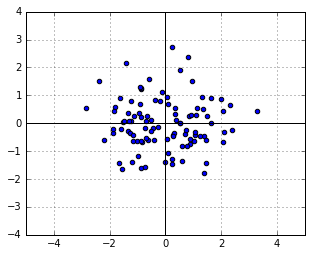
\includegraphics[width=7cm]{figs_hints_1.png}
\end{center}

We know from above that the likelihood of each point in this sample Is

\begin{equation}
  \label{symmetric_gaussian_probability}
  \text{P}(x)\propto\exp\left(-0.5\,\bm{x}^{\intercal}\bm{x}\right)
\end{equation}

Now let us apply a linear transformation $\bm{A}$ to the points, i.e. let $\bm{y} = \bm{Ax}$. Suppose that, for the sake of this example, $\bm{A}$ scales the vertical axis by 0.5 and then rotates everything by 30 degrees. We will get the following new cloud of points $\bm{y}$:

\begin{center}
  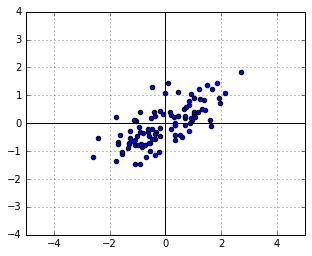
\includegraphics[width=7cm]{figs_hints_2.png}
\end{center}

What is the distribution of $\bm{y}$? Just substitute $\bm{x}=\bm{A}^{-1}\bm{y}$ into (\ref{symmetric_gaussian_probability}), to get:

\begin{equation}
  \label{eqn_gaussian_transformation}
  \begin{aligned}
    \text{P}(\bm{y}) &\propto \exp\left(-0.5\left(\bm{A}^{-1}\bm{y}\right)^{\intercal}\left(\bm{A}^{-1}\bm{y}\right)\right) \\
    &= \exp\left(-0.5\,\bm{y}^{\intercal}\left(\bm{A}\bm{A}^{\intercal}\right)^{-1}\bm{y}\right)
  \end{aligned}
\end{equation}

This is exactly the Gaussian distribution with covariance $\Sigma = \bm{A}\bm{A}^{\intercal}$. The logic works both ways: if we have a Gaussian distribution with covariance $\Sigma$, we can regard it as a \textit{distribution which was obtained by transforming the symmetric Gaussian by some} $\bm{A}$, and we are given $\bm{A}\bm{A}^{\intercal}$.\medskip

More generally, if we have \textit{any} data then, when we compute its covariance to be $\Sigma$, we can say that \textit{if our data were Gaussian}, then \textit{it could have been obtained} from a symmetric cloud using some transformation $\bm{A}$, and we just estimated the matrix $\bm{A}\bm{A}^{\intercal}$, corresponding to this transformation.\medskip

Note that we do not know the actual $\bm{A}$, and it is mathematically totally fait. There can be many different transformations of the symmetric Gaussian which result in the same distribution shape. For example, if $\bm{A}$ is just rotation by some angle, the transformation does not affect the shape of the distribution at all. COrrespondingly, $\bm{A}\bm{A}^{\intercal} = \bm{I}$ for all rotation matrices. When we see a unit covariance matrix we really do not know, whether is it the "originally symmetric" distribution, or a "rotated symmetric distribution". And we should not really care - those two are identical.\medskip

There is a theorem in linear algebra, which says that any symmetric matrix $\Sigma$ can be represented as:

\begin{equation}
  \label{eqn_sigma_decomposition}
  \Sigma = \bm{V}\bm{D}\bm{V}^{\intercal},
\end{equation}

where $\bm{V}$ is orthogonal (i.e. a rotation) and $\bm{D}$ is diagonal (i.e. a coordinate-wise scaling). If we rewrite it slightly, we will get:

\begin{equation}
  \Sigma = \left(\bm{V}\bm{D}^{\frac{1}{2}}\right)\left(\bm{V}\bm{D}^\frac{1}{2}\right)^{\intercal} = \bm{A}\bm{A}^{\intercal},
\end{equation}

where $\bm{A} = \bm{V}\bm{D}^{\frac{1}{2}}$. This, in simple words, means that \textit{any covariance matrix} $\Sigma$ could have been the result of transforming the data using a \textit{coordinate-wise scaling} $\bm{D}^{\frac{1}{2}}$ followed by a rotation V. Just like in our example with $\bm{x}$ and $\bm{y}$ above.

\paragraph{Principal Component Analysis}\mbox{}\\\\
Given the above intuition, PCA already becomes a very obvious technique. Suppose we are given some data. Let us assume \textit{(or "pretend")} it came from a normal distribution, and let us ask following questions:

\begin{enumerate}
  \item What could have been the rotation $\bm{V}$ and scaling $\bm{D}^{\frac{1}{2}}$, which produced our data from a symmetric cloud?
  \item What were the original, "symmetric-cloud" coordinates $\bm{x}$ before this transformation was applied?
  \item Which original coordinates were scaled the most by $D$ and this contribute most to the spread of the data now. Can we only leave those and throw the rest out?
\end{enumerate}

All of those questions can be answered in s straightforward manner if we decompose $\Sigma$ into $\bm{V}$ and $\bm{D}$ according to (\ref{eqn_sigma_decomposition}). But (\ref{eqn_sigma_decomposition}) is exactly the eigenvalue decomposition of $\Sigma$. I'll leave you to think for just a bit and you'll see how this observation lets you derive everything there it about PCA and more.

\paragraph{The Metric Tensor}\mbox{}\\\\
Bear me for just a bit more. On way to summarize the observation above is to say that we can (and should) regard $\Sigma^{-1}$ as a metric tensor. A metric tensor is just  fancy formal name for a matrix, which summarizes the \textit{deformation} of space. However, rather than claiming that in some sense determines a particular transformation $\bm{A}$ (which it does not, as we saw), we shall say that it affects the way we compute \textit{angles} and \textit{distances} in our transformed space.\medskip

Namely, let us redefine, for any two vectors $\bm{v}$ and $\bm{w}$, their inner product as:

\begin{equation}
  \langle\bm{v},\bm{w}\rangle_{\Sigma^{-1}} = \bm{v}^{\intercal}\Sigma^{-1}\bm{w}.
\end{equation}

To stay consistent we will also need to redefine the  \textit{norm} of any vector as.

\begin{equation}
  |\bm{v}|_{\Sigma^{-1}} = \sqrt{\bm{v}^{\intercal}\Sigma^{-1}\bm{v}},
\end{equation}

and the \textit{distance} between any two vectors as

\begin{equation}
  |\bm{v}-\bm{w}|_{\Sigma}^{-1} = \sqrt{(\bm{v}-\bm{w})^{\intercal}\Sigma^{-1}(\bm{v}-\bm{w})}.
\end{equation}

Those definitions now describe a kind of a "skewed world" of points. For example, a unit circle (a set of points with "skewed distance" 1 to the center) in this world might look as follows:

\begin{center}
  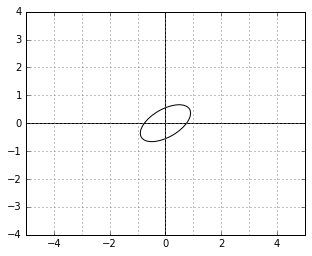
\includegraphics[width=7cm]{figs_hints_3.png}
\end{center}

And here is an example of two vectors, which are considered "orthogonal", a.k.a "perpendicular" in this strange world:

\begin{center}
  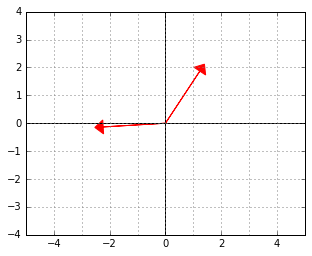
\includegraphics[width=7cm]{figs_hints_4.png}
\end{center}

Although it may look weird at first, note that the new inner product we defined is actually just the dot product of the "untransformed" originals of the vectors:

\begin{equation}
  \bm{v}^{\intercal}\Sigma^{-1}\bm{w} = \bm{v}^{\intercal}\bm{w} = 
  \bm{v}^{\intercal}\left(\bm{A}\bm{A}^{\intercal}\right)^{-1}\bm{w} =
  \left(\bm{A}^{-1}\bm{v}\right)^{\intercal}\left(A^{-1}\bm{w}\right),
\end{equation}

The following illustration might shed light on what is actually happening in this $\Sigma-$"skewed" world. Somehow "deep down inside", the ellipse thinks of itself as a circle and the two vectors behave as if they were $(2,2)$ and $(-2,2)$.

\begin{center}
  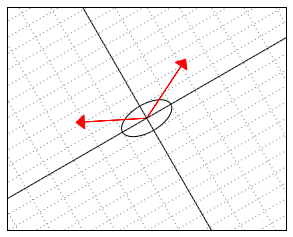
\includegraphics[width=7cm]{figs_hints_5.png}
\end{center}

Getting back to our example with the transformed points, we could now say that the point-cloud $y$ is actually a perfectly round and symmetric cloud "deep down inside", it just happens to live in a $skewed space$. The deformation of this space is described by the tensor $\Sigma^{-1}$ (which is, as we know), equal to $\left(\bm{A}\bm{A}^{\intercal}\right)^{-1}$. The PCA not becomes a method for analyzing the \textit{deformation of space}. How cool is that.

\paragraph{The Dual Space}\mbox{}\\\\
We are not done yed. There's one interesting property of "skewed" spaces worth knowing about. Namely, the elements of their dual space have a particular form. No worries, I'll explain in a second. \medskip

Let us forget the whole skewed space story for a moment, and get back to the usual inner product $\bm{W}^{\intercal}\bm{v}$. Think of this inner product as a function $f_{\bm{w}}(\bm{v})$, which takes a vector $\bm{v}$ and maos it to a real number, the dot product of $\bm{w}$ and $\bm{v}$. Regard the $\bm{w}$  here as the \textit{parameter ("weight vector")} of the function. If you have done any machine learning at all, you have certainly come across such \textit{linear functionals} over and over, sometimes in disguise. Now, the set of \textit{all possible linear functionals} $f_{\bm{w}}$ is known as the \textit{dual space} to your "data space".\medskip

Note that each linear functional is determined uniquely by the parameter vector $\bm{w}$, which has the same dimensionality as $\bm{v}$, so apparently the dual space is in some sense equivalent to your data space - just the interpretation is different. An element $\bm{v}$ of your “data space” denotes, well, a data point. An element $\bm{w}$ of the dual space denotes a function $f_{\bm{w}}$, which \textit{projects} your data points on the direction $\bm{w}$ (recall that if $\bm{w}$ is unit-length, $\bm{w}^{\intercal}\bm{v}$ is exactly the length of the perpendicular projection of $\bm{v}$ upon the direction $\bm{w}$). So, in some sense, if $\bm{v}$-s are “vectors”, w-s are “directions, perpendicular to these vectors”. Another way to understand the difference is to note that if, say, the elements of your data points numerically correspond to amounts in kilograms, the elements of $\bm{w}$ would have to correspond to “units per kilogram”. Still with me?\medskip

Let us not get back to the skewed space. If $\bm{v}$ are elements of a skewed Euclidean space with the metric tensor $\Sigma^{-1}$, is a function $f_{\bm{w}}(\bm{v}) = \bm{w}^{\intercal}\bm{v}$ an element of a dual space? Yes, it is, because, after all, it is a linear functional. However, the \textit{parameterization} of this function is inconvenient , because, due to the skewed tensor, we cannot interpret it as projecting vectors upon $\bm{w}$ nor can we say that $\bm{w}$ is an "orthogonal direction" (to a separating hyperline of a classifier, for example). Because, remember, in the skewed space it is not true that orthogonal vectors satisfy $\bm{w}^{\intercal}\bm{v} = 0$. Instead, they satisfy $\bm{w}^{\intercal}\Sigma^{-1}\bm{v} = 0$. Things would therefor look much better if we parameterized our dual space differently. Namely, by considering linear functionals of the form $f_{\bm{z}}^{\Sigma^{-1}}$. The new parameters $\bm{z}$ could now indeed be interpreted as an "orthogonal direction" and things overall would make more sense.\medskip

However when we work with actual machine learning models, we still prefer to have our functions in the form of dot product, i.e. $f_{\bm{w}}$, without any ugly $\Sigma$-s inside. What happens if we turn a "skewed space" linear functional from its natural representation into a simple inner product?

\begin{equation}
  f_{\bm{z}}^{\Sigma^{-1}}(\bm{v}) 
  = \bm{z}^{\intercal}\Sigma^{-1}\bm{v} 
  = \left(|sigma^{-1}\bm{z}\right)^{\intercal}\bm{v}
  = f_{\bm{w}}(\bm{v}),
\end{equation}

where $\bm{w}=\Sigma^{-1}\bm{z}$. (Note that we can lose the transpose because $\Sigma$ is symmetric).

What it means, in simple terms, is that when you fit linear models in a skewed space, your resulting weight vectors will always be of the form $\Sigma^{-1}\bm{z}$. Or, in other words, $|sigma^{-1}$ is a \textit{transformation, which maps from "skewed perpendiculars"} to \textit{"true perpendiculars"}. Let me show you what this means visually.\medskip

Consider again the two "orthogonal" vectors from the skewed world example above:

\begin{center}
  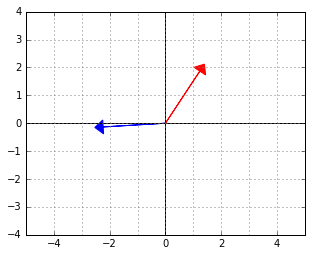
\includegraphics[width=7cm]{figs_hints_6.png}
\end{center}

Let us interpret the blue vector as an element of the \textit{dual space}. That is, it is the $\bm{z}$ vector in a linear functional $\bm{z}^{\intercal}\Sigma^{-1}\bm{v}$. The red vector is an element of the "data space", which would be mapped to 0 by this functional (because the two vectors are "orthogonal", remember).\medskip

For example, if the blue vector was meant to be a linear classifier, it would have its separating line along the red vector, just like that:

\begin{center}
  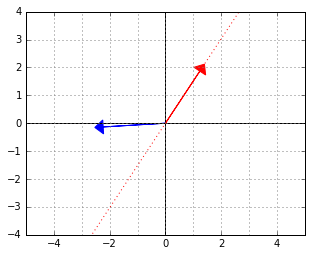
\includegraphics[width=7cm]{figs_hints_7.png}
\end{center}

If we now wanted to use this classifier, we could, of course, work in the "skewed space" and use the expression $\bm{z}^{\intercal}\Sigma^{-1}\bm{v}$ to evaluate the functional. However, why don't we find the actual \textit{normal} $\bm{w}$ to that red separating line so that we wouldn't eed to do extra multiplication every time we use the function?\medskip

It is not too hard to see that $\bm{w} = \Sigma^{-1}\bm{z}$ will give us that normal. Here it is, black arrow:\medskip

\begin{center}
  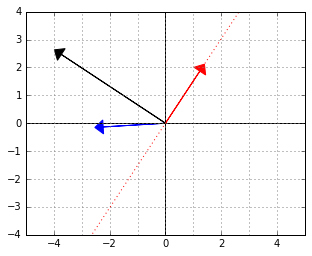
\includegraphics[width=7cm]{figs_hints_8.png}
\end{center}

Therefor, next time, whenever you see expressions like $\bm{w}^{\intercal}\Sigma^{-1}\bm{v}$ or $(\bm{v}-\bm{w})^{\intercal}\Sigma^{-1}(\bm{v}-\bm{w})$, remember that those are simply \textit{inner products and (squared) distances} in a skewed space, while $\Sigma^{-1}\bm{z}$ is a \textit{conversion from a skewed normal to a true normal}. Also remember that the "skew" was estimated by pretending that the data were normally distributed.\medskip 

Once you see it, the role of the covariance matrix in some methods like the Fisher's discriminant or Canonical correlation analysis might become much more obvious.

\paragraph{The Dual Space Metric Tensor}\mbox{}\\\\
"But wait", you should say here. "You have been talking about expressions like $\bm{w}^{\intercal}\Sigma^{-1}\bm{v}$ all the time, while things like $\bm{w}^{\intercal}\bm{v}$" are also quite common in practice. What about those?"\medskip

Hopefully you know enough now to suspect that $\bm{w}^{\intercal}\Sigma\bm{v}$ is again an inner product or a squared norm in some deformed space, just not the "internal data metric space", what we considered so far. What space is it? It turns out it is the "internal \textit{dual} metric space". That is , whilst the expression $\bm{w}^{\intercal}\Sigma^{-1}\bm{v}$ denoted the "new inner product" between the points, the expression $\bm{w}^{\intercal}\Sigma\bm{v}$ denotes the "new inner product" between the \textit{parameter} vectors. Let us see why it is so.\medskip

Consider an example again. Suppose that out space transformation $\bm{A}$ scaled by all points by 2 along $x$ axis. The point $(1,0)$ becomes $(2,0)$, the point $(3,1)$ becomes $(6,1)$ etc. Think of it as changing the units of measurement - before we measured the $x$ axis in kilogram, and not we measure it in pounds. Consequently, the norm of the point $(2,0)$ according to the new metric, $|(2,0)|_{\Sigma^{-1}}$ will be 1, because 2 pounds is still just a kilogram "deep down inside". \medskip

What should happen to the parameter \textit{("direction")} vectors due to this transformation? Can we say that the parameter vector $(1,0)$ also got scaled to $(2,0)$ and that the norm of the parameter vector $(2,0)$ is now therefore also 1? No! Recall that if our initial data denoted kilograms, our dual vectors must have denoted “units per kilogram”. After the transformation they will be denoting “units per pound”, correspondingly. To stay consistent we must therefore convert the parameter vector (”1 unit per kilogram”, 0) to its equivalent (“0.5 units per pound”,0). Consequently, the norm of the parameter vector $(0.5,0)$ in the new metric will be 1 and, by the same logic, the norm of the dual vector $(2,0)$ in the new metric must be 4. You see, the “importance of a parameter/direction” gets scaled inversely to the “importance of data” along that parameter or direction.\medskip

More formally, it $\bm{x}' = \bm{A}\bm{x}$, then

\begin{equation}
  \begin{aligned}
    f_{w}(\bm{x}) &= \bm{w}^{\intercal}\bm{x} = \bm{w}^{\intercal}\bm{A}^{-1}\bm{x}' \\
    &= \left(\left(\bm{A}^{-1}\right)^{\intercal}\right)^{\intercal}\bm{x}' = f_{(A^{-1})^{\intercal}\bm{w}}(\bm{x}').
  \end{aligned}
\end{equation}

This means that the transformation $\bm{A}$ of the data points implies the transformation $\bm{B}:=\left(\bm{A}^{-1}\right)$ of the dual vectors. The metric tensor for the dual space must thus be:

\begin{equation}
\left(\bm{B}\bm{B}^{\intercal}\right)^{-1} = \left(\left(\bm{A}^{-1}\right)^{\intercal}\bm{A}^{-1}\right)^{-1} = \bm{A}\bm{A}^{\intercal} = \Sigma.
\end{equation}

Remember the illustration of the "unit circle" in the $|sigma^{-1}$ metric? This is how the unit circle looks in the corresponding $\Sigma$ metric. It is rotated by the same angle, but it is stretched in the direction where it was squished before.

\begin{center}
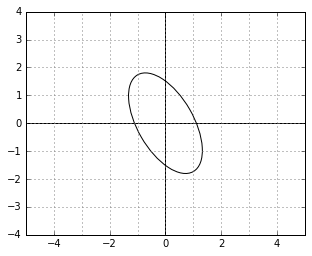
\includegraphics[width=7cm]{figs_hints_9.png}
\end{center}

Intuitively, the norm ("importance") of the dual vectors along the direction in which the data was stretched by $\bm{A}$ becomes proportionally large (note that the "unit circle" is, on the contrary, "squished" along those directions).\medskip

But the "stretch" of the space deformation in any direction can be measured by the variance of the data.It is therefore not a coincidence that $\bm{w}^{\intercal}\Sigma\bm{w}$ is exactly the variance of the data along the direction $\bm{w}$ ($assuming |\bm{w}| = 1$).

\paragraph{The Covariance Estimate}\mbox{}\\\\
Once we start viewing the covariance metric as a transformation-driven metric tensor, many things become clearer, but one things becomes extremely puzzling: \textit{why is the inverse covariance of the data a good estimate for that metric tensor}? After all, it it not obvious that $\bm{X}^{\intercal}\bm{X}/n$  (where $\bm{X}$ is the data matrix) must be related to the $\Sigma$ is the distribution equation $\exp\left(-0.5\,\bm{x}^{\intercal}\Sigma^{-1}\bm{x}\right)$.\medskip

Here is one possible way to see the connection. Firstly, let us take it for granted that if $\bm{X}$ is sampled from a symmetric Gaussian, then $\bm{X}^{\intercal}\bm{X}/n$ is, on average, a unit matrix. This has nothing to do with transformations, but just a consequence of pairwise independence of variables in the symmetric Gaussian.\medskip

Now, consider the transformed data, $\bm{Y} = \bm{X}\bm{A}^{\intercal}$ (vectors in the data matrix are row-wise, hence the multiplication on the right with a transpose). What is the covariance estimate of $Y$?

\begin{equation}
  \bm{Y}^{\intercal}\bm{Y}/n = \left(\bm{X}\bm{A}^{\intercal}\right)^{\intercal}\bm{X}\bm{A}^{\intercal}/n = \bm{A}\left(\bm{X}^{\intercal}\bm{X}\right)\bm{A}^{\intercal}/n \approx \bm{A}\bm{A}^{\intercal},
\end{equation}

the familiar tensor. \medskip

This is a place where one could see that a covariance matrix may make sense outside the context of a Gaussian distribution, after all. Indeed, if you assume that your data was generated from any distribution $\mathcal{P}$ with uncorrelated variables of unit variance and then transformed using some matrix $\bm{A}$, the expression $\bm{X}^{\intercal}\bm{X}/n$ will still be an estimate of $\bm{A}\bm{A}^{\intercal}$, the metric tensor for the corresponding (dual) space deformation.\medskip

However, note that out of \textit{all} possible initial distributions $\mathcal{P}$, the normal distribution is exactly the one with the maximum entropy, i.e. the “most generic”. Thus, if you base your analysis on the mean and the covariance matrix (which is what you do with PCA, for example), you could just as well assume your data to be normally distributed. In fact, a good rule of thumb is to remember, that whenever you even \textit{mention} the word "covariance matrix", you are implicitly fitting a Gaussian distribution to your data.

\end{document}


